% !TEX root = mythesis.tex

%==============================================================================
\chapter{NA64 Experimental Setup}
\label{sec:setup}
%==============================================================================
\begin{figure}[h!]
\centering
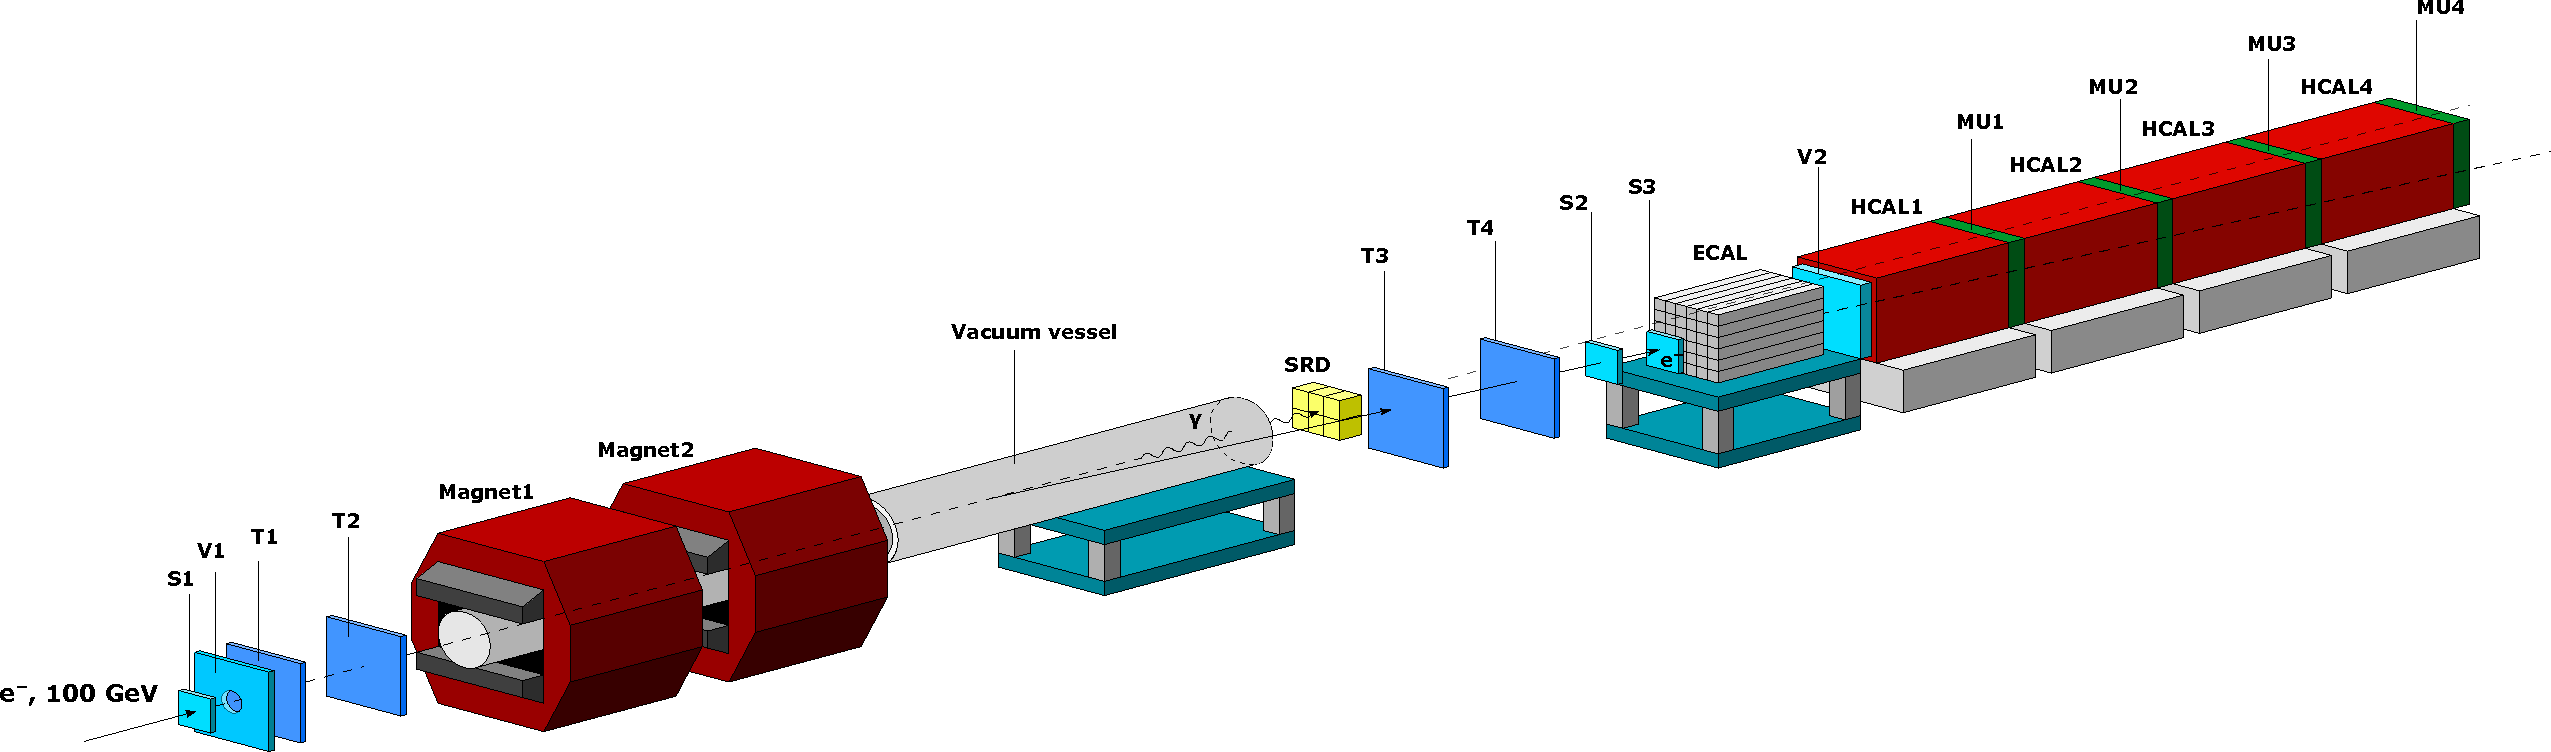
\includegraphics[width=\textwidth]{thesis_figures/Invisible_3d_setup.png}
\caption{Invisible mode setup~\cite{Banerjee:2016tad}}
\label{fig:Invisible_mode_setup}
\end{figure}

NA64 is a beam dump fixed-target experiment located at the H4 beam line of the Super Proton Synchrotron (SPS) at CERN. The objective of the detector is to look for rare dark matter candidates, primarily Dark Photons $A'$. $A'$ is supposed to be emitted via a process similar to bremsstrahlung $e^-Z\rightarrow e^- Z A'$. The experiment is not a permanent fixture and has been in operation since March, 2016. Since it's approval the setup has taken data a total of four times which included a two week test run in 2016 and four weeks of data taking each in 2016, 2017 and 2018. Each year the setup has slightly varied to account for different beam energies and expected background.

The SPS provides a primary proton beam of $400~\mathrm{GeV/c}$ with $\simeq 10^{12}$ protons per spill which is then converted to electrons by incidence on a beryllium target. The $e^-$ beam is in the momentum range $50-150~\mathrm{GeV/c}$ with a maximal intensity $\simeq 10^{7}$ per SPS spill of 4.8s. The provided high-energy $e^-$ beam with the large luminosity was needed since the $A'$ couples very weakly to the SM. The beam is then characterized by passing it through scintillators (S1-S3),veto ($V_1$), two dipole magnets with an integral magnetic field of $\simeq 7~\mathrm{Tm}$ and trackers (MM-section(\ref{sec:MM}), GEM-section(\ref{sec:GEM}) contained in tracking stations (T1-T4) which measure the $e^-$ beam momenta to a 1\% precision~\cite{article_beam_purity}. Additionally the combination of magnets followed by a 15m long vacuum vessel and a PbSc synchrotron radiation detector (SRD) acted as a filter to reject low energy electrons and hadrons that might be present in the beam and would contribute to the overall background. They were separated by putting a cut on the amount of synchrotron radiation energy deposited by the respective particle~\cite{Gninenko:2013rka}. The beam is then allowed to hit the electromagnetic calorimeter (ECAL) which acts as an active target. The ECAL consisted of 6x6 Shashlik-type modules each with 40 radiation lengths ($\mathrm{X_0}$) of which the initial 4$\mathrm{X_0}$ is employed as a separate preshower(PS) detector. The ECAL had a resolution of $\delta E_{ECAL}/E_{ECAL} \simeq 0.1 \sqrt{E_{ECAL}[\text{GeV}]}$~\cite{Banerjee:2016tad}.
The combined information achieved by studying the shower and the SRD signal helped in suppressing the hadron contamination in the beam to a remaining fraction of $ \lesssim 10^{-6}$~\cite{Depero:2017mrr}. A combination of Veto($V_2$) and hadronic calorimeter(HCAL) is situated downstream of the ECAL. They serve as a veto against muons, neutrals like high energy photons or hadrons produced in the target ECAL. The HCAL consisted of four modules ($\text{HCAL}_{1-4}$) separated by muon counters ($MU_{1-4}$) and were slightly shifted along the beam with each module consisting of 3x3 cells adding up to a total of $\simeq$30 nuclear interaction length ($\lambda_{int}$). The HCAL had a resolution of $\delta E_{HCAL}/E_{HCAL} \simeq 0.6 \sqrt{E_{HCAL}[\text{GeV}]}$~\cite{Banerjee:2016tad}.

\begin{figure}[t!]
\centering
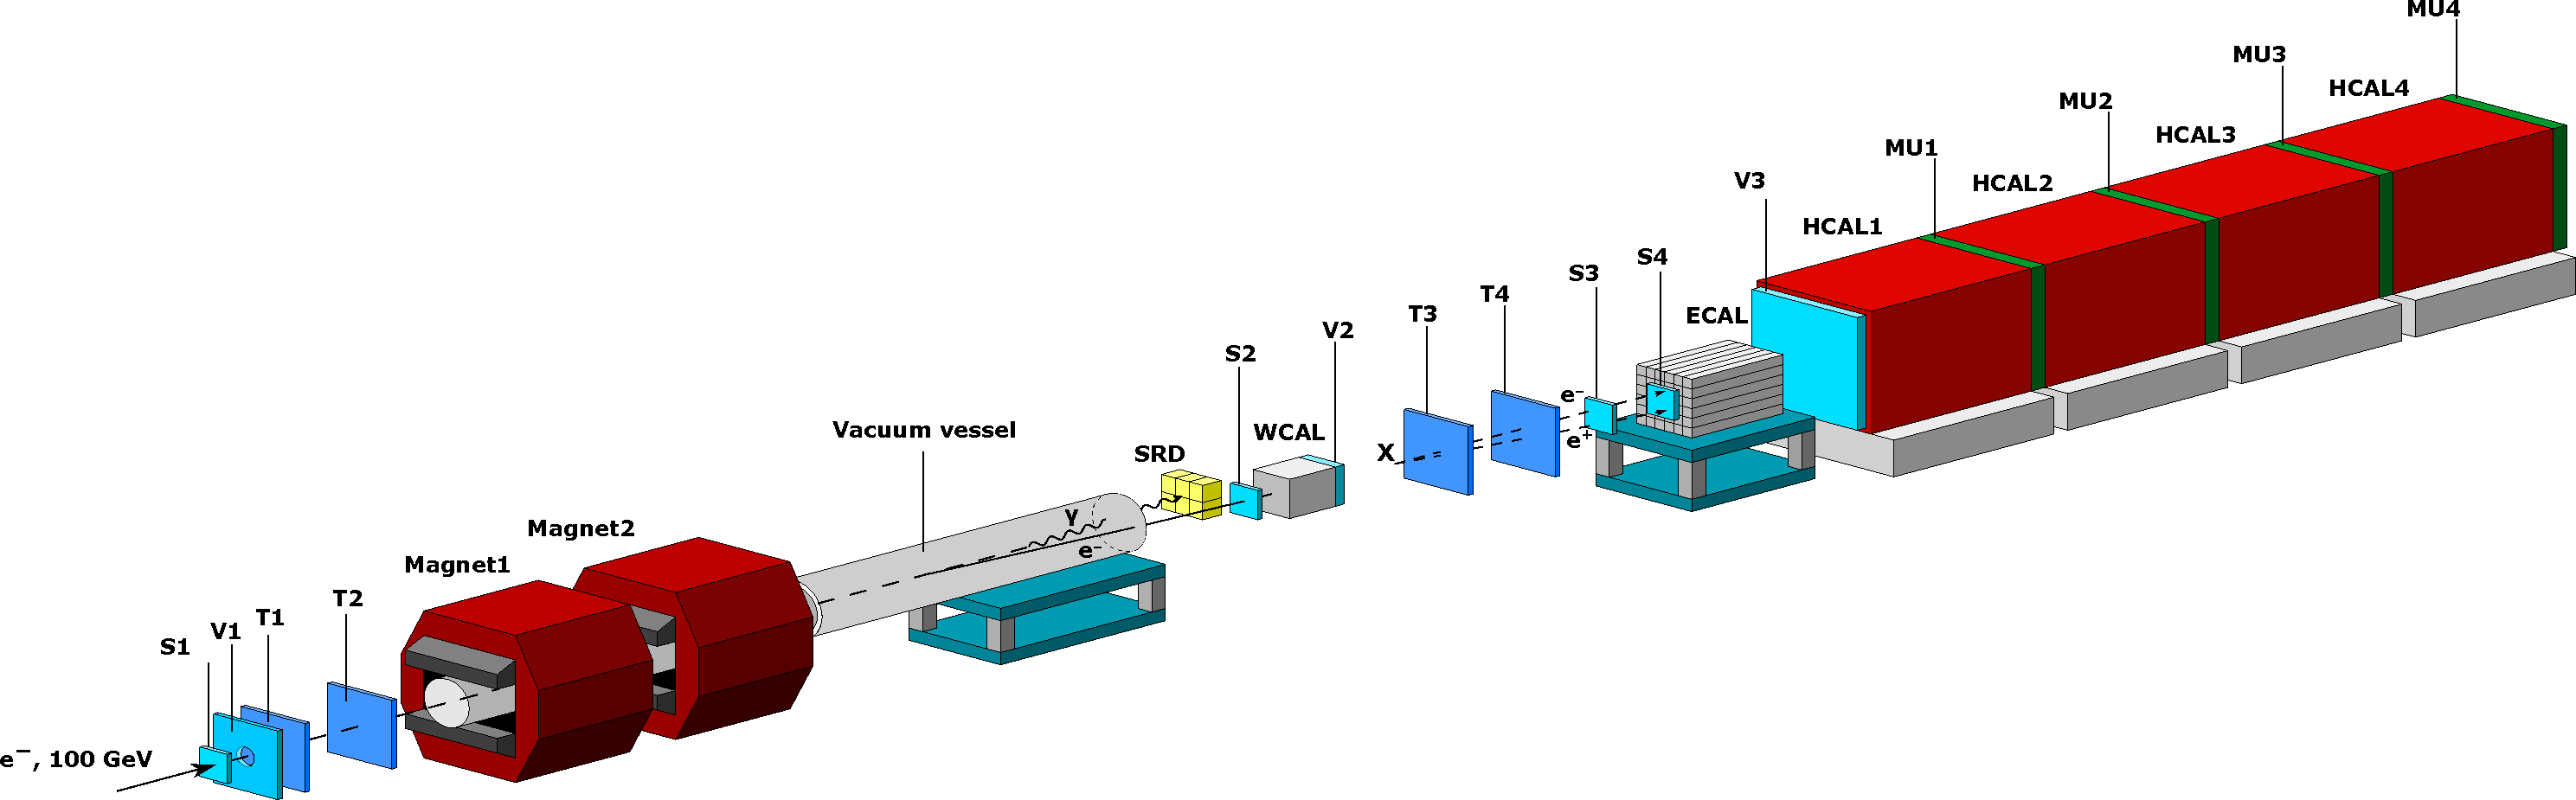
\includegraphics[width=\textwidth]{thesis_figures/Visible_3d_setup.png}
\caption{Visible mode setup 2017~\cite{Banerjee_2018}}
\label{fig:Visible_mode_setup}
\end{figure}

\begin{figure}[t!]
\centering
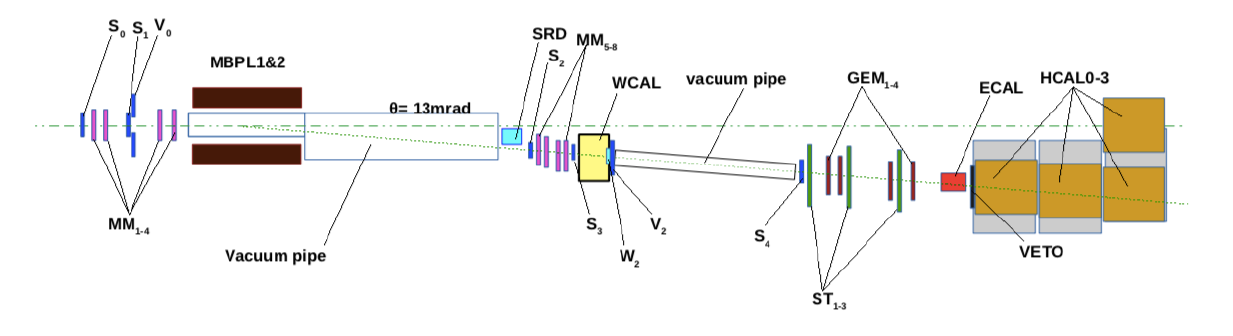
\includegraphics[width=\textwidth]{thesis_figures/visible_mode_newest.png}
\caption{Visible mode setup 2018-top view~\cite{Gninenko:2677228}}
\label{fig:Visible_mode_setup_side}
\end{figure}

The above setup works well for the \textit{invisible mode}($10^{-4} \lesssim \epsilon \lesssim 10^{-3}$, $m_{A'} \lesssim 1 \text{GeV}$) but requires modification for the search of $A'(X)$ in the \textit{visible mode}($10^{-4} \lesssim \epsilon \lesssim 10^{-3}$, $m_{A'} \lesssim 100 \text{MeV}$). To search for the visible decays a short tungsten calorimeter (WCAL) and a veto ($V_2$) were added right after the vacuum pipe and before the second set of tracking detectors (fig.(\ref{fig:Visible_mode_setup})). The size of the WCAL was selected so that the leakage of particles is small and the sensitivity to short lifetimes is maximized. The distance between the WCAL and the ECAL for the visible mode searches was slightly varied(2.5m->5.6m) between 2017 and 2018 which allowed for the installation of a 3.1m long vacuum tube to create better spacing between the ECAL and WCAL for a better angular resolution to increase the sensitivity to X17 bosons~\cite{Banerjee_2018}. A WCAL catcher was also installed in 2018 to prevent any leakage. Additionally the beam momentum was increased from 100GeV to 150 GeV in 2018 and one of the tracking station consisting of two MicroMegas (MM) was also shifted upstream of the WCAL. Counter ($W_2$) and straw detectors ($\text{ST}_{1-3}$) were also tested during the 2018 beam period(fig.(\ref{fig:Visible_mode_setup_side})). Both \textit{invisible} and \textit{visible} mode setups were also used to look for rare SM events that involve a photon decaying to a dimuon pair via bremsstrahlung $e^-Z\rightarrow e^-Z\gamma;\gamma\rightarrow \mu^{+} \mu^{-} $. Comparing these rare events, which were obtained from real data, to our Monte Carlo(MC) simulated sample helped in estimating the validity and efficiency of our MC simulation~\cite{Gninenko:2677228}.

In summary, NA64 tries to estimate and tag the beam $e^-s$ using a combination of trackers, SRD and ECAL/WCAL, uses the said ECAL/WCAL as an active target and then collects the residue of the interaction in the downstream HCAL/ECAL+HCAL. It also utilizes the hard bremsstrahlung photon to dimuon conversion as a measuring stick for the reliability of the MC simulations. The reactions of interest were attempted to be observed with a combination of hardware and software triggers depending on the expected signature of the decay mode for $A'$.

\textbf{Invisible Mode:}
$A'\rightarrow \chi \overline{\chi}$ signature:
\begin{flalign*}
  Beam(p\simeq 100~\text{GeV}),\\
  E_{ECAL+PS}(< 100~\text{GeV}),\\
  V_2(< E^{th}_{V}\simeq 1~\text{MIP}),\\
  E_{HCAL}(< E^{th}_{HCAL}\simeq 1~\text{GeV}).
\end{flalign*}

\textbf{Visible Mode:}
$A'\rightarrow e^+ e^-$ signature:
\begin{flalign*}
  Beam(p\simeq 150~\text{GeV}), \\
  E_{WCAL}(< 150~\text{GeV}), \\
  E_{WCAL+ECAL+PS}(\simeq 150~\text{GeV}), \\
  V_2(> E^{th}_{V}\simeq 1~\text{MIP}), \\
  V_3(< E^{th}_{V}), \\
  E_{HCAL}(< E^{th}_{HCAL}\simeq 1~\text{GeV}).
\end{flalign*}







%%% Local Variables:
%%% mode: latex
%%% TeX-master: "mythesis"
%%% End:
